
\documentclass[conference]{IEEEtran}
\usepackage{amsmath,amssymb,booktabs,array}
\usepackage[T1]{fontenc}
\usepackage{tikz}
\usetikzlibrary{arrows.meta,positioning,shapes.geometric}
\begin{document}
% Anonymous CMT review version. Restore author names and affiliations for camera-ready submission if required.

\title{Single-Step Contextual PPO for Multi-Resource and Multi-KPI Optimization in AI-Native 6G RAN}

\author{\IEEEauthorblockN{Dr. Rao S. Yenamandra}
\IEEEauthorblockA{DigitalTwinSim\\
Email: raosy@digitaltwinsim.com}}
\maketitle

\begin{abstract}
AI-native operation is an important direction for future IMT-2030/6G radio access networks (RANs), where learning-based functions can participate directly in closed-loop observation, decision, and resource optimization. Proximal Policy Optimization (PPO) is commonly presented for multi-step Markov Decision Processes (MDPs), but a useful class of RAN optimization problems can instead be posed as repeated single-step contextual decisions. This paper proposes a single-step contextual PPO framework in which a multi-KPI RAN context is mapped to independent or joint control actions over multiple radio resources. Candidate controls include physical resource block (PRB) allocation, transmit power, spectrum or bandwidth assignment, and MIMO configuration. Each control may be decreased, held, or increased within feasible operating limits. The objective is a multi-KPI reward emphasizing cell throughput, cell-edge throughput, Jain fairness, and a normalized resource/energy-efficiency index. Because each optimization call terminates after the immediate reward and the next context is treated as exogenous, no discounted future return, value bootstrap from a successor state, or generalized advantage estimation is required. The PPO probability ratio, clipped surrogate objective, critic baseline, entropy regularization, and end-to-end neural-network backpropagation are retained. An illustrative synthetic PRB-allocation example is presented to demonstrate the single-step learning procedure. It represents one feasible instance of the proposed framework; the broader multi-resource formulation is a general proposal whose expected KPI effects are described qualitatively rather than claimed as measured gains. The resulting context-to-policy-to-constrained-action loop is positioned as a lightweight AI-native RRM framework for future 6G RAN, while remaining applicable to advanced 5G deployments.
\end{abstract}

\begin{IEEEkeywords}
6G, AI-native RAN, Proximal Policy Optimization, contextual bandit, reinforcement learning, RAN optimization, multi-resource control, multi-KPI optimization, RRM.
\end{IEEEkeywords}

\section{Introduction}
Future IMT-2030/6G systems are expected to place increasing emphasis on ubiquitous intelligence and AI/ML-enabled network operation \cite{itu2030}. In this paper, \emph{AI-native RAN} denotes an architecture in which learning-based inference and closed-loop optimization are designed as integral RAN capabilities rather than being added only as an external advisory function. This motivates resource-management loops in which RAN measurements form the context, an AI policy selects a feasible action, and the resulting KPI response provides immediate feedback. The proposed method is an AI-native-RAN-compatible RRM framework; it is not claimed to constitute a complete standardized 6G architecture.

RAN performance is governed by several coupled radio resources and operating parameters. PRB allocation directly affects scheduled bandwidth and load; transmit power influences link quality, coverage, interference, and energy use; spectrum or bandwidth assignment changes available capacity; and MIMO configuration changes the number of spatial streams and associated radio-resource cost. Optimizing any one variable in isolation can improve one KPI while degrading another. A useful RAN optimizer should therefore observe several KPIs jointly and select one or more resource-control actions according to a multi-objective reward.

This paper proposes a single-step contextual PPO formulation for that purpose. On each optimization call, the controller observes a snapshot of RAN conditions, selects an independent or joint action over multiple controllable resources, observes the immediate post-action KPI outcome, and terminates the episode. The next presented context is assumed to be generated independently or by an exogenous network process not caused by the previous action. Under this assumption, the problem is a contextual bandit rather than a full temporal MDP.

The contribution is a general multi-resource formulation rather than a claim that all candidate controls have been experimentally validated. The paper retains the defining PPO update machinery---the old/new policy probability ratio, clipped surrogate objective, learned baseline, entropy regularization, and gradient-based neural-network learning---while removing trajectory-dependent return estimation, successor-state bootstrapping, and generalized advantage estimation (GAE). An illustrative synthetic PRB-allocation example is presented as one concrete demonstration of the single-step PPO mechanism.


\begin{figure*}[t]
\centering
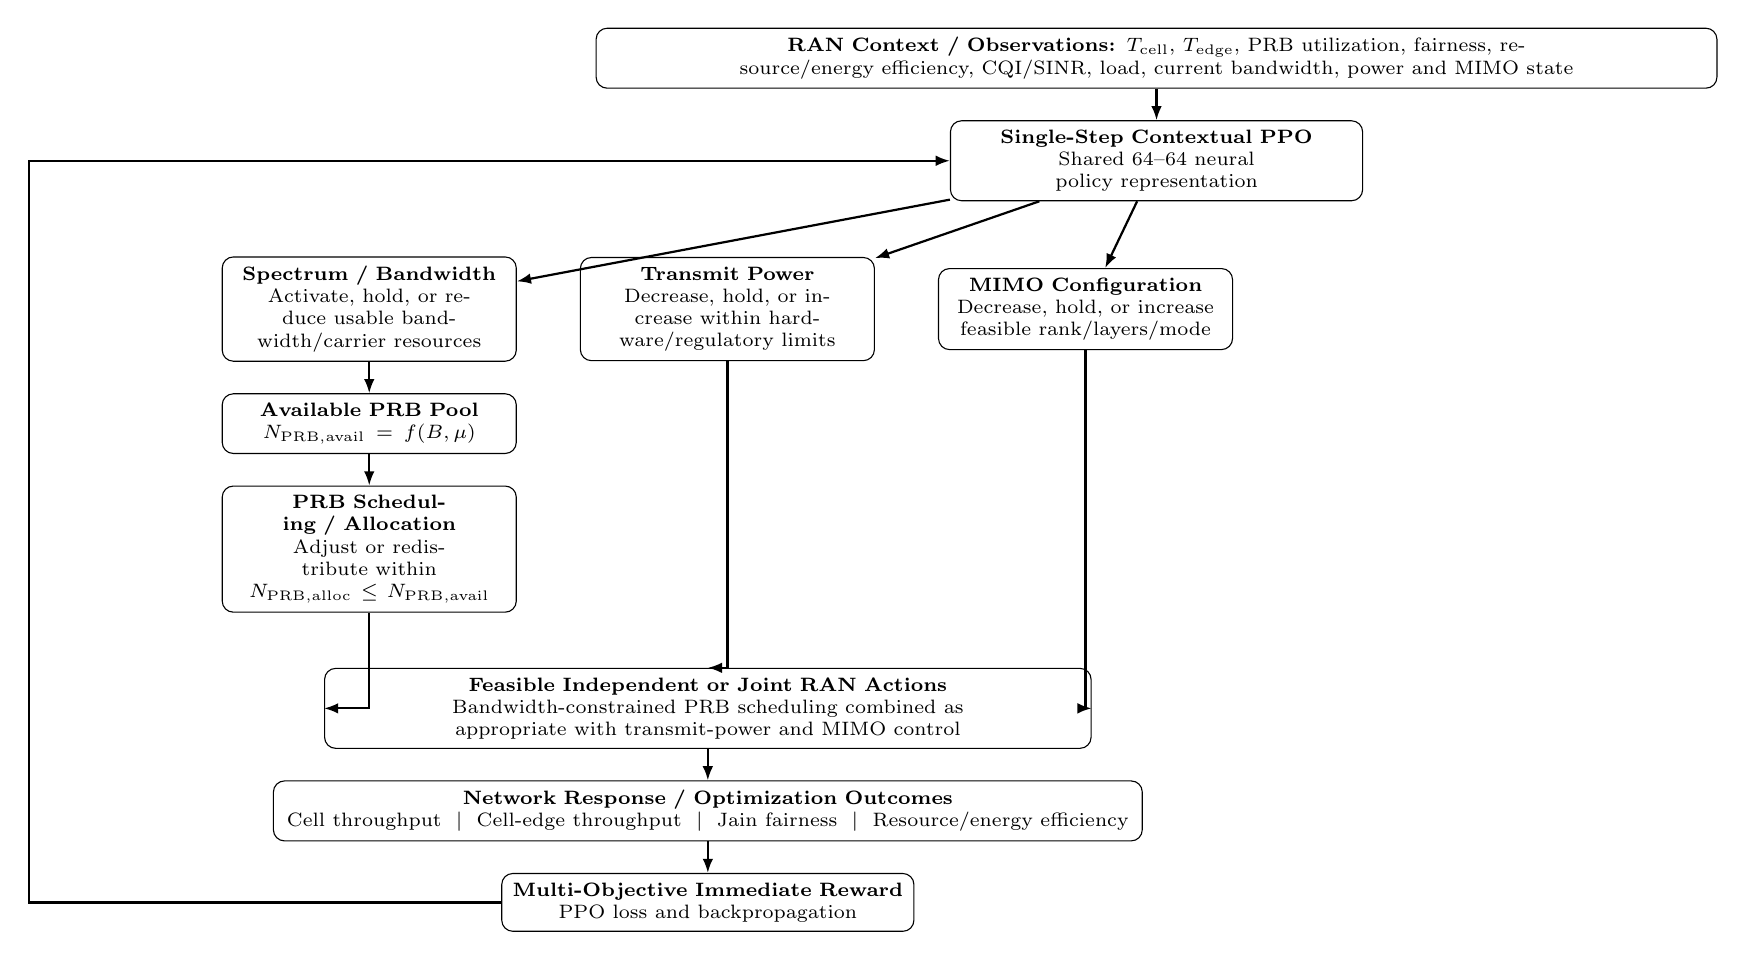
\begin{tikzpicture}[
node distance=4mm and 8mm,
box/.style={draw, rounded corners, align=center, minimum height=7mm, font=\scriptsize},
arrow/.style={-{Latex[length=1.8mm]}, thick}
]
\node[box, text width=14.0cm] (ctx) {\textbf{RAN Context / Observations:}
$T_{\rm cell}$, $T_{\rm edge}$, PRB utilization, fairness, resource/energy efficiency, CQI/SINR, load, current bandwidth, power and MIMO state};
\node[box, text width=5.0cm, below=of ctx] (ppo) {\textbf{Single-Step Contextual PPO}\\Shared 64--64 neural policy representation};

\node[box, text width=3.5cm, below left=7mm and 55mm of ppo] (bw) {\textbf{Spectrum / Bandwidth}\\Activate, hold, or reduce usable bandwidth/carrier resources};
\node[box, text width=3.5cm, right=8mm of bw] (pwr) {\textbf{Transmit Power}\\Decrease, hold, or increase within hardware/regulatory limits};
\node[box, text width=3.5cm, right=8mm of pwr] (mimo) {\textbf{MIMO Configuration}\\Decrease, hold, or increase feasible rank/layers/mode};

\node[box, text width=3.5cm, below=of bw] (pool) {\textbf{Available PRB Pool}\\$N_{\rm PRB,avail}=f(B,\mu)$};
\node[box, text width=3.5cm, below=of pool] (prb) {\textbf{PRB Scheduling / Allocation}\\Adjust or redistribute within\\$N_{\rm PRB,alloc}\leq N_{\rm PRB,avail}$};

\node[box, text width=9.5cm, below=7mm of prb, xshift=43mm] (resp) {\textbf{Feasible Independent or Joint RAN Actions}\\Bandwidth-constrained PRB scheduling combined as appropriate with transmit-power and MIMO control};
\node[box, text width=10.8cm, below=of resp] (kpi) {\textbf{Network Response / Optimization Outcomes}\\Cell throughput $\;|\;$ Cell-edge throughput $\;|\;$ Jain fairness $\;|\;$ Resource/energy efficiency};
\node[box, text width=5.0cm, below=of kpi] (rew) {\textbf{Multi-Objective Immediate Reward}\\PPO loss and backpropagation};

\draw[arrow] (ctx) -- (ppo);
\draw[arrow] (ppo) -- (bw);
\draw[arrow] (ppo) -- (pwr);
\draw[arrow] (ppo) -- (mimo);
\draw[arrow] (bw) -- (pool);
\draw[arrow] (pool) -- (prb);
\draw[arrow] (prb.south) |- (resp.west);
\draw[arrow] (pwr.south) |- (resp.north);
\draw[arrow] (mimo.south) |- (resp.east);
\draw[arrow] (resp) -- (kpi);
\draw[arrow] (kpi) -- (rew);
\draw[arrow] (rew.west) -| ++(-6.0,0) |- (ppo.west);
\end{tikzpicture}
\caption{Proposed constrained multi-resource single-step contextual PPO flow. Bandwidth and numerology determine the available PRB pool; PRB scheduling/allocation is bounded by that pool, while transmit power and MIMO are separately constrained controls that may be optimized independently or jointly.}
\label{fig:flow}
\end{figure*}

\section{Multi-KPI Context}
At decision round $t$, the controller observes a context vector
\begin{equation}
\mathbf{s}_t=[T_{\rm cell},T_{\rm edge},U_{\rm PRB},F,E_{\rm eff},C_{\rm radio}],
\end{equation}
where $T_{\rm cell}$ is cell downlink throughput, $T_{\rm edge}$ is cell-edge throughput, $U_{\rm PRB}$ is PRB utilization or a derived utilization-efficiency measure, $F$ is Jain's fairness index, $E_{\rm eff}$ is a normalized resource/energy-efficiency index, and $C_{\rm radio}$ denotes additional radio context needed to make a feasible decision, such as CQI/SINR distribution, active-user load, available bandwidth, current transmit-power operating point, and current MIMO configuration.

The four principal outcome KPIs used in the proposed multi-objective optimization are
\begin{equation}
\mathbf{k}_t=[T_{\rm cell},T_{\rm edge},F,E_{\rm eff}].
\end{equation}
PRB utilization and other radio measurements may be used as context or constraints rather than being forced to behave as monotonic reward terms. This separates what the controller \emph{observes} from what it is explicitly asked to \emph{improve}.

\section{Multi-Resource Action Space}
The proposed control vector may be written as
\begin{equation}
\mathbf{a}_t=
[a_{\rm BW},a_{\rm PRB},a_{\rm P},a_{\rm MIMO}],
\end{equation}
but these controls are not all physically independent. In particular, spectrum/bandwidth and numerology determine the available PRB pool,
\begin{equation}
N_{\rm PRB,alloc}\leq N_{\rm PRB,avail}(B,\mu),
\end{equation}
where $B$ is the active channel bandwidth and $\mu$ denotes the numerology. PRB scheduling therefore redistributes or adjusts allocation only within the available PRB pool; it cannot increase PRBs beyond the bandwidth-dependent limit.

For a simple discrete proposal, each feasible control direction can be represented by resource-specific actions analogous to DECREASE, HOLD, and INCREASE. For spectrum/bandwidth, this means reducing, holding, or increasing active bandwidth or carrier resources when spectrum and configuration permit. For PRBs, it means reducing, holding, or increasing the scheduled allocation within $N_{\rm PRB,avail}$, or redistributing PRBs among users. For transmit power, it means changing the permitted power operating point within regulatory and hardware limits. For MIMO, it means changing an allowed rank, number of spatial layers, or antenna mode when supported by channel conditions and UE/gNB capability.

Resources may be controlled independently or jointly, but every joint action is subject to feasibility constraints. For example, a request to increase scheduled PRBs is admissible only if the active bandwidth provides unused PRBs; otherwise the bandwidth/carrier action must first or jointly enlarge the available pool. Joint control can therefore select combinations such as increasing usable bandwidth and then allocating additional PRBs, reducing transmit power while maintaining PRB allocation, or increasing MIMO rank while holding bandwidth. Four nominal three-way controls yield up to $3^4=81$ combinations, but infeasible combinations are removed or masked. A factorized multi-discrete policy with one output head per control can reduce output complexity while retaining constrained joint actions.

The stochastic policy is
\begin{equation}
\mathbf{a}_t\sim\pi_\theta(\mathbf{a}|\mathbf{s}_t).
\end{equation}
Feasibility masks can exclude actions that violate spectrum availability, maximum transmit power, supported MIMO rank, minimum scheduling requirements, or other operator constraints.

\section{Multi-KPI Reward}
The proposed immediate reward is a weighted multi-objective function
\begin{equation}
r_t=R(\mathbf{s}_t,\mathbf{a}_t)
=w_T\hat T_{\rm cell}
+w_E\hat T_{\rm edge}
+w_F F
+w_\eta E_{\rm eff}
-P_{\rm viol},
\end{equation}
where the throughput terms are normalized, $E_{\rm eff}$ is a dimensionless normalized resource/energy-efficiency index, and $P_{\rm viol}$ penalizes infeasible or undesirable operating regions. The weights can be selected according to operator objectives.

The reward is intentionally multi-KPI because the resources are coupled. Increasing transmit power may improve edge throughput but reduce energy efficiency or increase interference. Increasing bandwidth or PRBs may raise throughput but can become inefficient under light load. Increasing MIMO rank can improve capacity when channel conditions support additional layers but may provide little benefit or incur extra cost when they do not. PPO therefore learns the action or joint action that maximizes the weighted outcome for the current context rather than applying a fixed direction of change to every resource.

\section{Single-Step PPO Formulation}
Because the episode terminates after the immediate reward, no future reward exists to discount and no discount factor is required for the single-step return. A critic estimates the expected immediate reward,
\begin{equation}
V_\phi(\mathbf{s}_t)\approx
\mathbb{E}_{\mathbf{a}\sim\pi_\theta}
[R(\mathbf{s}_t,\mathbf{a})],
\end{equation}
and the advantage is
\begin{equation}
A_t=r_t-V_\phi(\mathbf{s}_t).
\end{equation}
There is no successor-state bootstrap and no GAE.

The probability ratio is
\begin{equation}
\rho_t(\theta)=
\frac{\pi_\theta(\mathbf{a}_t|\mathbf{s}_t)}
{\pi_{\theta_{\rm old}}(\mathbf{a}_t|\mathbf{s}_t)}.
\end{equation}
The clipped surrogate objective retains the standard PPO form \cite{ppo}:
\begin{equation}
L^{\rm CLIP}(\theta)=
\mathbb{E}_t\!\left[
\min\!\left(
\rho_tA_t,
\mathrm{clip}(\rho_t,1-\epsilon,1+\epsilon)A_t
\right)\right].
\end{equation}
The critic loss is
\begin{equation}
L^{\rm VF}(\phi)=
\mathbb{E}_t[(V_\phi(\mathbf{s}_t)-r_t)^2],
\end{equation}
and the combined minimization loss is
\begin{equation}
L=-L^{\rm CLIP}+c_1L^{\rm VF}-c_2H[\pi_\theta].
\end{equation}

A lightweight policy architecture is proposed using two hidden layers of 64 neurons each. The actor uses a shared 64--64 feed-forward representation followed by separate constrained action heads for spectrum/bandwidth, PRB scheduling/allocation, transmit power, and MIMO configuration. A corresponding 64--64 critic produces the scalar immediate-reward baseline. Backpropagation updates all trainable weights. The 64--64 choice is a proposed compact architecture rather than a claim of optimal network size, and the qualitative multi-resource KPI expectations in this paper are not attributed to that architecture without empirical validation.

\section{Expected KPI Effects of Multi-Resource Control}
Table I summarizes the expected first-order KPI tendencies of the candidate controls. These are engineering expectations, not measured numerical results. Actual effects depend on channel quality, interference, load, scheduler constraints, hardware capability, and the simultaneous settings of the other resources.

\begin{table*}[t]
\caption{Expected Qualitative KPI Effects of Candidate RAN Control Actions}
\centering
\scriptsize
\setlength{\tabcolsep}{3.5pt}
\renewcommand{\arraystretch}{1.15}
\begin{tabular}{p{2.0cm}p{1.55cm}p{2.55cm}p{2.55cm}p{2.45cm}p{3.0cm}}
\toprule
Resource/control & Action & Cell throughput & Cell-edge throughput & Fairness & Resource/energy efficiency\\
\midrule
PRB allocation &
Dec./Hold/Inc. &
More useful PRBs can raise throughput; excess allocation can waste resources. &
Can improve when edge users receive more scheduling opportunity. &
Can improve when allocation corrects user imbalance; can degrade if concentrated on strong users. &
Improves when allocation matches load; can degrade with over-allocation or congestion.\\
\addlinespace
Transmit power &
Dec./Hold/Inc. &
Better SINR may raise throughput, but added interference can limit net gain. &
Often benefits coverage-limited or edge users. &
Can improve when weak users become schedulable; excess interference can reverse the benefit. &
Lower power can improve efficiency; higher power is useful only when KPI gain offsets energy/interference cost.\\
\addlinespace
Spectrum / bandwidth &
Dec./Hold/Inc. &
More usable bandwidth generally raises capacity when demand exists. &
May improve if additional spectrum is usable at the edge. &
Can improve by relieving congestion and increasing scheduling flexibility. &
Best when bandwidth activation follows demand; lightly loaded extra bandwidth may reduce efficiency.\\
\addlinespace
MIMO configuration &
Dec./Hold/Inc. rank/mode &
More spatial layers can raise throughput when rank and SINR support them. &
Benefit depends on edge-channel rank and link quality. &
Can improve if spatial resources are distributed across users; may favor strong users if unconstrained. &
Higher rank can improve bits/resource under favorable channels but may add RF/baseband cost.\\
\bottomrule
\end{tabular}
\end{table*}

The expected objective is therefore not ``increase every resource.'' The desired PPO behavior is context dependent. Under congestion it may increase bandwidth or MIMO capability while redistributing PRBs; under weak edge conditions it may favor power or scheduling changes; under light load it may reduce power, bandwidth activation, or MIMO complexity while maintaining throughput. The policy can trade small reductions in one KPI for larger weighted improvements in the others, subject to constraints.

\section{Independent Versus Joint Optimization}
Independent resource actions simplify attribution and reduce action-space size, but they can miss interactions. For example, increasing transmit power and MIMO rank simultaneously may have a different effect from applying either change alone. Joint actions allow PPO to exploit such coupling, but they increase the number of combinations and the amount of training data required.

A practical compromise is a shared contextual encoder with factorized action heads. Each head outputs probabilities for DECREASE, HOLD, and INCREASE for one resource. The joint action probability can be represented as the product of the conditional head probabilities when the factorization assumption is used. More advanced variants can add autoregressive or coupled heads if interactions require explicit dependence among actions.

\section{Illustrative PRB-Allocation Example}
An illustrative synthetic PRB-allocation example is presented to show how the proposed single-step PPO procedure can learn a context-dependent policy. It uses an eMBB-only 6 GHz, 200 MHz scenario \cite{38104}, a five-dimensional normalized KPI context, and three PRB actions \{REDUCE, HOLD, INCREASE\}. This example demonstrates the single-step probability-ratio, clipping, critic, and backpropagation procedure for one constrained resource-control case. The transmit-power, spectrum/bandwidth, and MIMO controls are proposed extensions and are not assigned measured gains in this paper.

\begin{table}[t]
\caption{Illustrative Held-Out Reward: PRB-Only Case}
\centering\footnotesize
\begin{tabular}{lc}
\toprule
Policy & Mean reward\\
\midrule
Learned (greedy) & +0.502\\
Uniform random & +0.447\\
\bottomrule
\end{tabular}
\end{table}

The learned PRB-only policy improves aggregate reward by approximately 12\% relative to the uniform-random action baseline on 5,000 held-out contexts. This result should be interpreted only as evidence that the single-step PPO update learns a nontrivial context-to-action mapping in the illustrative environment. It is not a measured prediction of the gains that would result from the broader multi-resource proposal.

\section{Expected Benefits and Validation Requirements}
The proposed multi-resource formulation is expected to provide three main benefits. First, it can exploit complementary control mechanisms: throughput need not be improved only by consuming additional PRBs if bandwidth, MIMO configuration, or power provides a better tradeoff. Second, it can explicitly protect cell-edge performance and fairness through the reward rather than optimizing average throughput alone. Third, it can trade performance against normalized resource/energy efficiency, allowing the controller to hold or reduce unnecessary resources when demand is low.

No numerical percentage improvement is assigned to the proposed multi-resource controls in this paper because such values require an environment that models the causal response of all four resources, including interference, link adaptation, MIMO rank feasibility, spectrum availability, traffic load, and power consumption. Future validation should compare the proposed policy against deterministic HOLD, threshold-based control, proportional-fair scheduling, and other relevant baselines, and should report confidence intervals over multiple traffic and channel conditions.


\subsection{Small Language Model Extension}
Where sufficient local processing capability and storage are available, an open-source small language model (SLM) could alternatively be adapted as a policy representation for multi-resource RAN optimization. Such a model may be useful when the decision context extends beyond compact numerical KPIs to heterogeneous configuration information, operator policies, domain knowledge, or previously unseen operating conditions. However, the substantially larger memory footprint, computational demand, and inference latency of an SLM may make it less suitable for frequent or near-real-time control than the proposed lightweight 64--64 neural policy. Increased model size also does not inherently imply greater KPI improvement for a structured low-dimensional numerical control problem. A meaningful comparison should therefore evaluate an SLM and the lightweight PPO policy under identical RAN contexts, feasibility constraints, reward functions, and test scenarios.

\section{Single-Step Versus Full-MDP Scope}
The contextual-bandit reduction is appropriate only when each optimization call is treated as an independent decision and the selected action does not determine the next context used for learning. If power, bandwidth, MIMO, or scheduling decisions are allowed to create persistent state transitions, delayed effects, mobility-dependent consequences, or multi-interval resource commitments, the formulation should be extended to a full MDP with multi-step returns and appropriate value bootstrapping.

\section{Conclusion}
This paper proposes single-step contextual PPO as a general framework for multi-resource, multi-KPI optimization in an AI-native 6G RAN setting. The controller observes a RAN context, independently or jointly adjusts PRB allocation, transmit power, spectrum/bandwidth assignment, and MIMO configuration, and evaluates an immediate multi-objective reward based principally on cell throughput, cell-edge throughput, fairness, and normalized resource/energy efficiency. The formulation retains PPO clipping and neural-network backpropagation while eliminating trajectory machinery that is unnecessary for independent one-step decisions.

The expected advantage of the multi-resource formulation is not that every radio resource should be increased, but that the policy can learn which resource or combination should be decreased, held, or increased for the current network context. The illustrative PRB-allocation example demonstrates the single-step learning mechanism for one resource-control case; quantitative validation of the full multi-resource proposal remains future work. The framework therefore represents a lightweight path toward AI-native 6G RRM: AI participates directly in constrained resource decisions rather than merely advising a conventional optimizer. A complete 6G realization would additionally require standardized data and model interfaces, lifecycle management, assurance, security, distributed inference/training, and safe fallback mechanisms.

\begin{thebibliography}{00}
\bibitem{ppo} J. Schulman, F. Wolski, P. Dhariwal, A. Radford, and O. Klimov, ``Proximal Policy Optimization Algorithms,'' arXiv:1707.06347, 2017.
\bibitem{38104} 3GPP, ``NR; Base Station (BS) radio transmission and reception,'' 3GPP TS 38.104, Release 18.
\bibitem{itu2030} ITU-R, ``Framework and overall objectives of the future development of IMT for 2030 and beyond,'' Recommendation ITU-R M.2160-0, Nov. 2023.
\end{thebibliography}

\end{document}
